\documentclass[letterpaper,12pt]{article}

%\setlength{\parindent}{0in}
%\usepackage{fullpage} 
\usepackage{amsmath}
\usepackage{amssymb}
\usepackage{enumerate}
\usepackage{graphicx}
\usepackage[table]{xcolor}
\usepackage{dcolumn}
\oddsidemargin 0.0in
\textwidth 6.5in
\newcolumntype{.}{D{.}{.}{-1}}
\newcommand*{\myalign}[2]{\multicolumn{1}{#1}{#2}}

%opening
\title{Evolution and Military Adoption \\ of Commercial Smart Phones}
\author{Steve Mazza}
\date{September 3, 2012}

\begin{document}
\maketitle

\begin{abstract}
The evolution of commercial smart phones and subsequent early adoption by Department of Defense (DoD) is better understood by first looking at the technology.  After establishing a working description, we look at some of the market drivers that have shaped the evolution and high growth of the devices.  For a better understanding of the direction they are headed, we look at the technology and forces that came together to enable current smart phones.  We wrap up by discussing the different variants, rates of adoption and permutation, and provide a brief forecast for the ten year horizon contrasting civilian and military use.
\end{abstract}

% Make 2 parts per section: first about the technology in general and second about the Army's use of it.
\section*{Technology Description}
% Describe the technology and include pictures, drawings, or other illustrations as appropriate.
Smart phones are the result of the intersection of several mature and emerging consumer technologies including cellular, WiFi, Bluetooth, and near field communications (NFC) tightly coupled with various sensors such as accelerometer, global positioning system (GPS), compass, proximity, and touch.  The smart phone revolution started in early 2003 with the introduction of the BlackBerry Quark\footnote{Wikipedia, \emph{List of BlackBerry Products}, http://en.wikipedia.org/wiki/List\_of\_BlackBerry\_products (as of \today).}.  Fueled by consumer demand, Microsoft and Palm entered the market.  But it wasn't until Apple introduced the iPhone that the revolution fully took hold.  No longer just the tools of the business elite, now these devices were actively marketed to the average consumer -- equally at home in the boardroom and in your kid's backpack.

\section*{Technological Need}
% What are the needs the technology fulfills � think back to SE3100 when you did a capability needs analysis.  Define and/or model as appropriate the needs (wants) the technology fulfills.  What functions does the technology provide?  How does it fit into its environment?
More and more, our lives put us on the go.  In a consumer driven market, manufacturers respond to the needs of our lifestyles.  Whether for work or personal use, our smart phones span the distance from home, to the gym, to work, and are even with us on our commute time in between.  In the Army's case, warfighters' needs are not all that different and smart phones are finding a niche in stateside training commands, permanent CONUS duty stations, and at different echelons in theater from Division all the way down to the dismounted soldier on patrol.  

Key enablers of these devices both for the Army and for civilian use are the reduction in size, weight, power, and cost compared with carrying similar previous generation devices.  Prior to the introduction of the smart phone, the end user would need an MP3 player, a hand held GPS, a cellular phone, and a laptop in order to get the same functionality; the size, weight, power, and cost of which were all prohibitive.  Today, all of this functionality slips neatly into your pocket and costs less than \$500.00.

\section*{Evolution of the Technology}
% How has the technology evolved over its history?  Research when the technology was first introduced, how it was introduced, and its major milestones over the technology�s lifetime.
Started by Blackberry and fueled by unrelenting consumer demand, the history of the smart phone market has been marked by the introduction of several disruptive technologies.  As early as 1983, Motorola began commercial marketing of the DynaTAC 8000X.  

\begin{center}
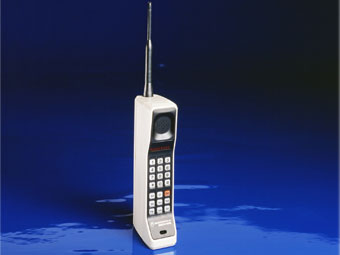
\includegraphics[scale=0.8]{images/dynaTac8000}
\end{center}

Cell phones continued to progress at a steady albeit slow pace through the introduction of the Palm Pilot in 1996 which, while it contained no cellular capability, brought together many other features of the personal organizer.  Interestingly, the pre-Jobs Apple Newton introduced in February, 1998, went almost completely unnoticed by consumers.  

\begin{center}
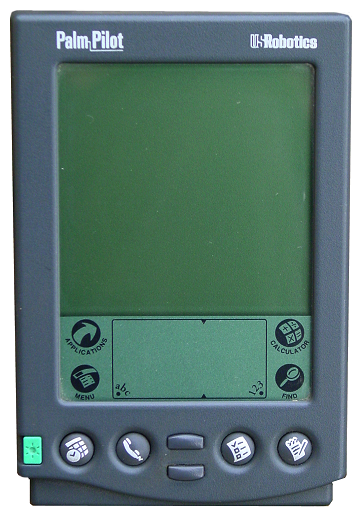
\includegraphics[scale=0.3]{images/Palmpilot5000}
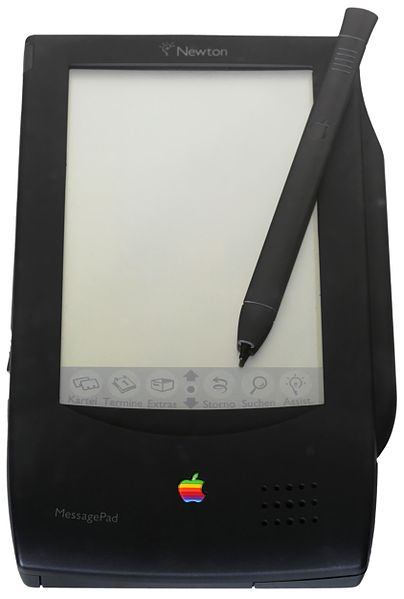
\includegraphics[scale=0.3]{images/Apple_Newton}
\end{center}

It wasn't until the introduction of the Blackberry Quark by Research In Motion (RIM) that consumer demand for an integrated cell phone and personal digital assistant (PDA) really caught hold.  RIM's rise to the top would prove to be as quick as its reign was short-lived.  Apple's introduction of the iPhone in early 2007 marked the greatest advance in this consumer technology and took the market by storm. 

\begin{center}
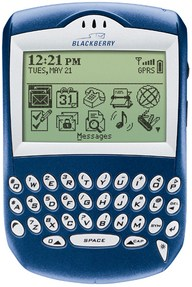
\includegraphics[scale=0.8]{images/blackberry_6200}
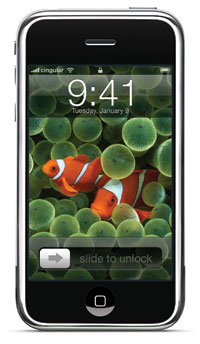
\includegraphics[scale=0.6]{images/apple-iphone}
\end{center}

Shortly thereafter, Google released the first commercial version of the Android operating system in September, 2008, code named \emph{Astro}.  Android continues to provide significant market pressure fueling continued innovation and lowering the barrier to market penetration.  By the end of 2010, Android became the world's leading smart phone platform\footnote{Wikipedia, \emph{Android (operating system)}, http://en.wikipedia.org/wiki/Android\_(operating\_system), (as of \today).}.

\section*{Technologically Enabling Advances}
% What technical advances in related or component technologies enable this technology?  What knowledge is associated with the development of the technology? (e.g., mechanical knowledge, nuclear, �)
Smart phone technology is really a system of systems, bringing together a cadre of sensors, cellular, and WiFi capability (plus more recently near field communications, or NFC) under an integrated and unified user interface which is facilitated by touch screen capability.  The technology enabling advances have principally been increases battery life, reductions in power draw, and the ability to produce inexpensive, high resolution capacitive touch screens.

It is arguable that Apple's introduction of the iPod in November, 2001\footnote{Wikipedia, \emph{iPod}, http://en.wikipedia.org/wiki/IPod, (as of \today).}, that did more to fuel the commercial smart phone industry than any other single technological advance.  It paved the way for consumers to expect more diverse capabilities from their portable electronic devices and allowed industry to see beyond the previous limitation of the traditional cellular phone.

Given the current climate of constrained defense budgets as well as consumer belt tightening, we cannot completely decouple the technological advances from the economic enablers as we attempt to understand the rapid growth of the commercial smart phone market.  As well as the important technological leaps forward mentioned above, it is an economy of scale in manufacturing and marketing that have provided a price point that is just within the threshold for consumer spending.  Without this important market force, amortizing the significant research and development spending in the private sector by companies like Apple, Nokia, Samsung, HTC, RIM, and others, the unit cost would be significantly higher thus increasing the barrier to adoption for military use.

\section*{Variants of the Technology}
% Are there variants of the same technology?  If so, what are the differences/similarities of those variants?  (e.g., automobile technology, there are variants in engine type, transmission, etc.).  Variants indicate either different needs, different prioritization of needs, or different solution approaches to the same problem.

\section*{Technology Diffusion}
% Explain the mechanisms and timing of how the technology diffused through the market, military, or society?  How long did it take to be adopted?

\section*{Growth Rate}
% What has been the growth rate of the technology?  Define appropriate measures of effectiveness and/or performance and determine its growth rate.  For example, for automobiles you could look at mpg, average service life, reliability, and other relevant measures.

\section*{Forecast}
% Forecast likely scenarios of where the technology will be 10 � 20 years from today; and/or create a technology roadmap of where the main stakeholders would likely want the technology to be.


\end{document}